% TU Delft Beamer template
% Author: Maarten Abbink
% Delft University of Technology
% March 2014
% Version 2.0
% Based on original version 1.0 of Carl Schneider
\documentclass[spanish]{beamer}
\usepackage{calc}
\usepackage[absolute,overlay]{textpos}
\mode<presentation>{\usetheme{tud}}
\usepackage[utf8]{inputenc}
\usepackage[spanish]{babel}


\newtheorem{examplefirst}{Modelo}
\newtheorem{examplesecond}{Modelo}

\newenvironment<>{examplefirst}[1][]{%
\setbeamercolor{block title example}{fg=white,bg=red!75!black}%
  \begin{example}#2[#1]}
  {\end{example}}


\newenvironment<>{examplesecond}[1][]{%
  \setbeamercolor{block title example}
  {fg=white,bg=blue!75!black}%
  \begin{example}#2[#1]}
  {\end{example}}


%%%%%%%%%%%%%%%%%%%%%%%%%%%%%%%%%%%%
\usepackage{lmodern}
\usepackage[T1]{fontenc}
\usepackage[utf8]{inputenc}
\usepackage{babel}

\makeatletter
\def\th@mystyle{%
    \normalfont % body font
    \setbeamercolor{block title example}{bg=orange,fg=white}
    \setbeamercolor{block body example}{bg=orange!20,fg=black}
    \def\inserttheoremblockenv{exampleblock}
  }
\makeatother
\theoremstyle{mystyle}
\newtheorem*{obs}{Observación}
\newtheorem*{conc}{Conclusión}


\title[COMIA 2015]{\normalsize  Clasificación automática de la orientación semántica de opiniones mediante características lingüísticas}
%\subtitle
\institute[F. Ciencias-UNAM]{\small Facultad de Ciencias, UNAM.}

\author{\href{mailto:alonsop@ciencias.unam.mx}{Alonso Palomino Garibay} y \href{mailto:sngh@fciencias.unam.mx}{Sofía N. Galicia-Haro}}
\date{28 de Mayo de 2015}

% Insert frame before each subsection (requires 2 latex runs)
\AtBeginSubsection[] {
	\begin{frame}<beamer>\frametitle{\titleSubsec}
	    \scriptsize
		\tableofcontents[currentsection,currentsubsection]  % Generation of the Table of Contents
	\end{frame}
}
% Define the title of each inserted pre-subsection frame
\newcommand*\titleSubsec{\large Siguiente sección}
% Define the title of the "Table of Contents" frame
\newcommand*\titleTOC{COMIA 2015 - Contenidos}

% define a symbol which can be removed if you don't need it
\newcommand{\field}[1]{\mathbb{#1}}
\newcommand{\Zset}{\field{Z}}

\begin{document}

{
% remove the next line if you don't want a background image
\usebackgroundtemplate{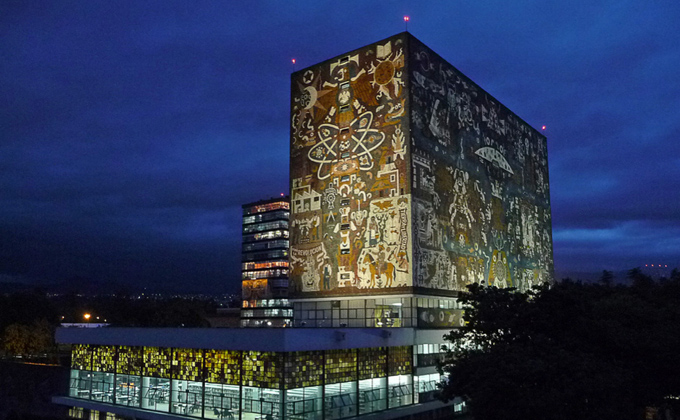
\includegraphics[width=\paperwidth,height=\paperheight]{images/background-titlepage.jpg}}%
\setbeamertemplate{footline}{\usebeamertemplate*{minimal footline}}
\frame{\titlepage}
}

{\setbeamertemplate{footline}{\usebeamertemplate*{minimal footline}}
\begin{frame}\frametitle{\titleTOC}
    \scriptsize
	\tableofcontents
\end{frame}
}

%Aqui empieza el contenido de la presentacion


\section{Introducción}
\subsection{Introducción}

%%%%%%%%%%%%%%Diapositiva 1
\begin{frame}\frametitle{Introducción - Minería de opiniones}

\begin{figure}
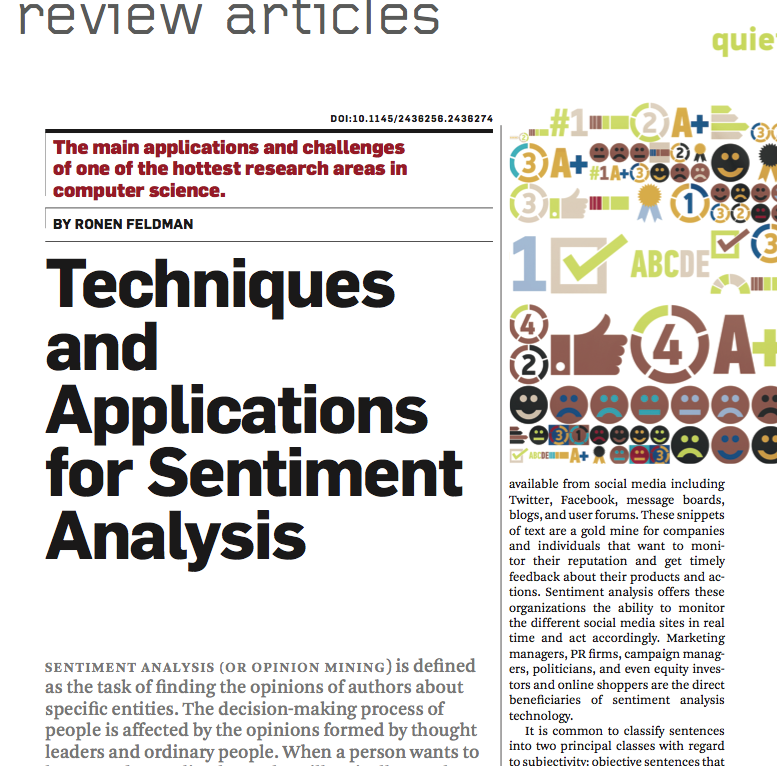
\includegraphics[scale=0.2]{images/cacm.png}
\caption{ Communications of the ACM, Vol. 56 No. 4, Paginas 82-89}
\end{figure}

%Años recientes han sido testigos de un interés en métodos computacionales para identificar sentimiento, desde minería de opiniones hasta detección de subjetividad.
  
    
    %\begin{example}
	%	\begin{minipage}{0.6\textwidth}
			% insert picture (pdf file)
	%		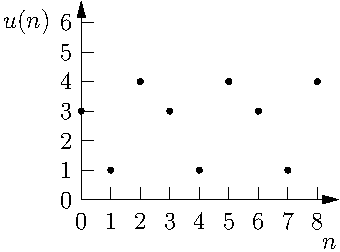
\includegraphics{images/ex1_periodic_number.pdf}
	%	\end{minipage}
	%	\centering{$u(n)=[3,1,4]_n$}
	%\end{example}
\end{frame}
%%%%%%%%%%%%%% Fin de la Diapositiva 1

%%%%%%%%%%%%%% Diapositiva 2
\begin{frame}\frametitle{Introducción - Minería de opiniones}

\begin{columns}[T] % contents are top vertically aligned
\begin{column}[T]{6cm} % each column can also be its own environment
     \setbeamertemplate{itemize items}[square]
  \begin{itemize}
  \item <2->Existe una enorme cantidad de comentarios de libre acceso en la Web, para productos y servicios.
  \begin{itemize}
  \item <3->Recurso valioso para la \alert{toma de decisiones}
  
  \end{itemize}
  
  \item <4->Monitoreo de redes sociales, rastreo de reseñas de clientes, encuestas, \alert{bussines analitycs}.
  
  \item <5->Las empresas pueden mejorar sus ventas
  
  \end{itemize}
     \end{column}
     \begin{column}[T]{5cm} % alternative top-align that's better for graphics
          
\includegraphics[height=4cm,scale=0.1]{images/imagen_1.jpg}
     \end{column}
     \end{columns}
     


%	\begin{definition}
%		Let $n$ be a discrete variable, i.e. $n\in\Zset$.
%		A 1-dimensional periodic number is a function that depends periodically on $n$.
%		$$
%		u(n)=
%		[u_0,u_1,\ldots,u_{d-1}]_n=
%		\begin{cases}
%			u_0 & \mbox{ if $n\equiv 0 \pmod d$} \\
%			u_1 & \mbox{ if $n\equiv 1 \pmod d$} \\
%			\vdots \\
%			u_{d-1} & \mbox{ if $n\equiv d-1 \pmod d$}
%		\end{cases}
%		$$
%		$d$ is called the period.
%	\end{definition}
\end{frame}
%%%%%%%%%%%%%% Fin de la diapositiva 2

%%%%%%%%%%%%%% Diapositiva 3
\begin{frame}\frametitle{Introducción  - Minería de opiniones}

	\begin{definition}
		\textbf{Minería de opiniones:}\\ Se refiere al estudio computacional de opiniones, sentimientos, evaluaciones, actitudes, apreciaciones, afecciones, puntos de vista, emociones y subjetividades expresadas en texto.
	\end{definition}
	\begin{center}
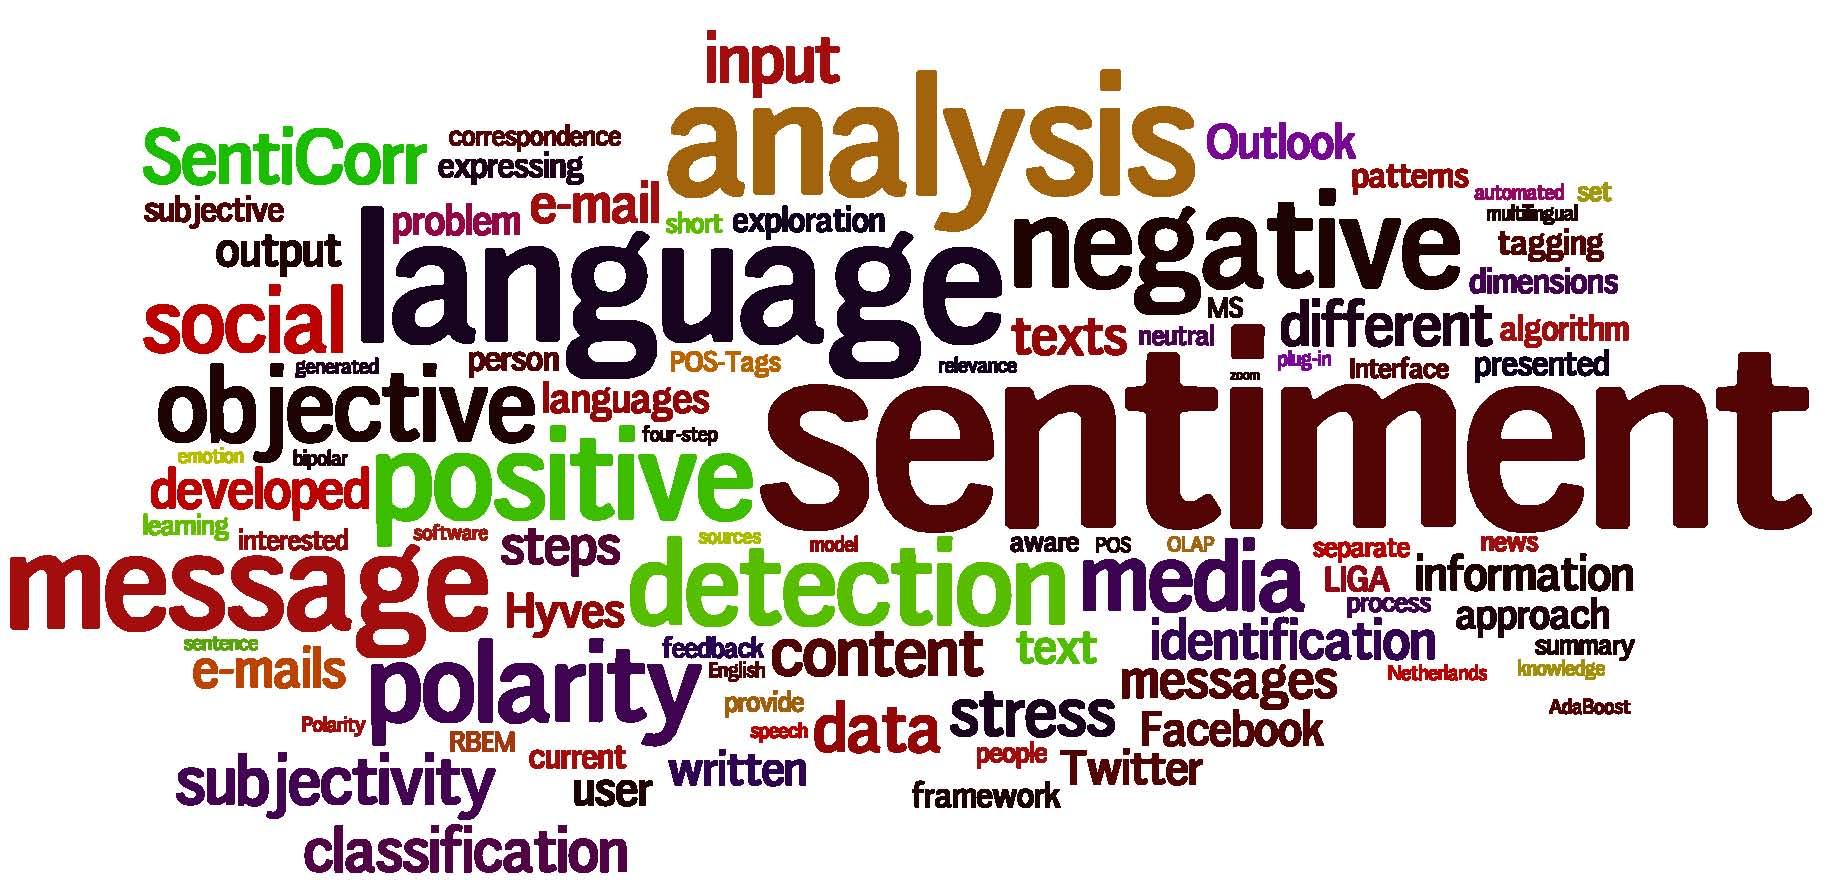
\includegraphics[height=3.5cm,scale=1]{images/sent_cloud.jpg}
\end{center}

\end{frame}
%%%%%%%%%%%%%% Fin de la Diapositiva 3

%%%%%%%%%%%%%% Diapositiva 4
\begin{frame}\frametitle{Introducción  - Minería de opiniones}


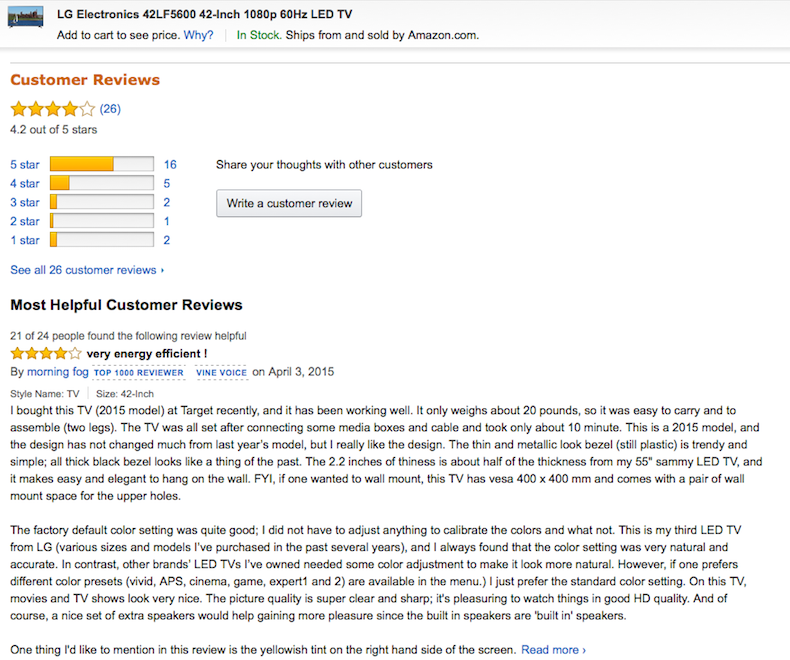
\includegraphics[width=\textwidth]{images/review_amazon.png}

\end{frame}
%%%%%%%%%%%%%% Fin de la Diapositiva 4



%%%%%%%%%%%%%% Diapositiva 5
\begin{frame}\frametitle{Introducción  - Minería de opiniones}

%\begin{itemize}
%\item La minería de opiniones intenta clasificar opiniones de forma automática en función de lo que cada autor expresa.

Subtareas dentro de la \alert{minería de opiniones}:

\begin{itemize}


\item <2->Turney (2002)
\begin{itemize}
\item Determinó la orientación semántica a partir de \alert{bigramas} (¿Positivo o Negativo?).
\end{itemize}


\item <3->Bo Pang et al (2008):
\begin{itemize}
\item Identificación de opiniones, polaridad del sentimiento, resumir de forma automática la orientación de una opinión.
\end{itemize}

\item <4->Liu Bing et al (2010)
\begin{itemize}
\item análisis de sentimiento en oraciones de comparación, detección de SPAM, detección de opiniones neutrales y engañosas.


\end{itemize}

\end{itemize}




\end{frame}
%%%%%%%%%%%%%% Fin de la Diapositiva 5




%\begin{frame}\frametitle{Introducción  - Subsection 1 - Page 3}
	%this is too big.
%	\begin{example}
%		\centering
%		{
%		$$
%		\begin{array}{rcl}
%			f(n)
%			&=&
%			-\left[\frac{1}{2},\frac{1}{3}\right]_n n^2
%%			\\
%			&=&
%			\begin{cases}
%				-\frac{1}{3} n^2 +3n-2
%				& \text{ if $n\equiv 0 \pmod 2$} \\
%				-\frac{1}{2} n^2 +3n-1
%				& \text{ if $n\equiv 1 \pmod 2$}
%			\end{cases}
			% &=&
			% -\frac{n^2}{2}+3n-1
			% -\left\{ \frac{n}{2} \right\}
			% \left( \frac{2}{3}n^2+2
			% \right)
%		\end{array}
%		$$
%		\begin{minipage}{0.4\textwidth}
%			% insert picture (pdf file)
%			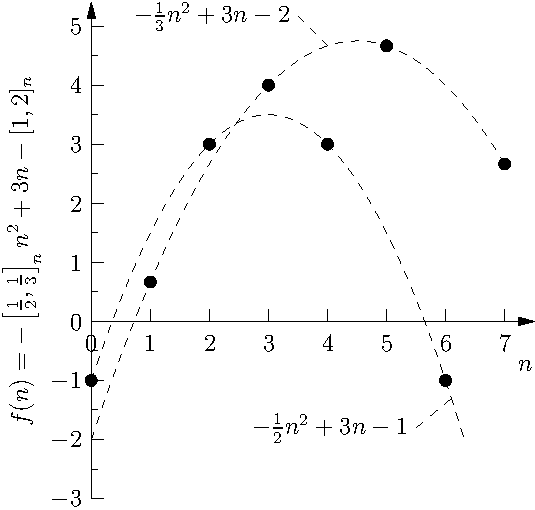
\includegraphics[width=\textwidth]{images/ex2_quasi_polynomial.pdf}
%		\end{minipage}
%		}
%	\end{example}
%\end{frame}


%%%%%%%%%%%Diapositiva 6
\section{Materiales empleados y conocimiento lingüístico considerado}

\subsection{Corpus de opiniones}

\begin{frame}\frametitle{\normalsize Corpus de opiniones}
	%\begin{alertblock}{Alertblock}
	%	This page gives an example with numbered bullets (enumerate)\\
	%	in an "Example" window:\\
	%\end{alertblock}
	
	%\begin{example}
	%	Discrete domain $\Rightarrow$ evaluate in each point\\
	%	Not possible for\\
	%	\begin{enumerate}
	%		\item <1-> parametric domains
	%		\item <2-> large domains (NP-complete)
	%	\end{enumerate}
	%\end{example}
	
\begin{columns}[T] % contents are top vertically aligned


\begin{column}[T]{5cm} % alternative top-align that's better for graphics

\includegraphics[height=4.5cm,scale=0.1]{images/ciao.png}
     \end{column}


\begin{column}[T]{6cm} % each column can also be its own environment
Corpus de trabajo extraído de \textbf{ciao.es}\footnote{\textit{\tiny Sofía N. Galicia-Haro y Alexander Gelbukh (2014).}}

\setbeamertemplate{itemize items}[square]
\begin{itemize}
\item <2->2800 opiniones de lavadoras en Español.
\item <3->Tamaño promedio por lexemas es de 345.
\item <4->El numero total de lexemas de la colección es de 845,280.
\end{itemize}
\end{column}
     \end{columns}
     
\end{frame}

%%%%%%%%%%%%%%%%%%%%%%%% fin diapositiva 6

%%%%%%%%%%%%%%%%%%%%%%%%%Diapositiva 7
\begin{frame}\frametitle{\large Corpus de opiniones}
\begin{figure}
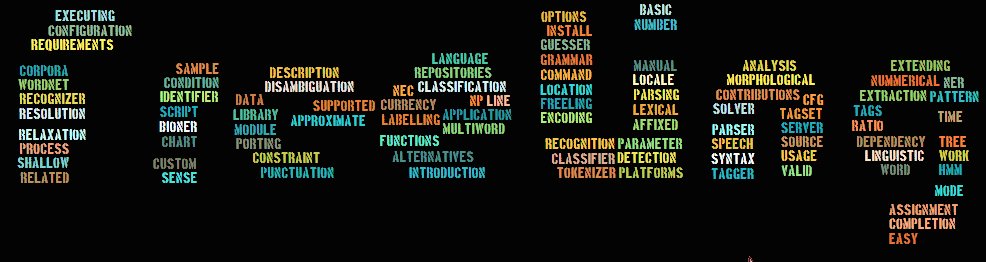
\includegraphics[scale=0.30]{images/freeling.png}
\caption{Lluís Padró and Evgeny Stanilovsky.
FreeLing 3.0 \textit{(2012)}}
\end{figure}
\begin{itemize}
\item <2-> La colección fue anotada con su \alert{lema} y \alert{categoría gramatical}.
\item <3-> Se utilizaron un conjunto de etiquetas para representar la información morfológica de las palabras.
\item <4->Este conjunto de etiquetas se basa en las etiquetas propuestas por el grupo EAGLES para la anotación morfosintáctica de lexicones y corpus para todas las lenguas europeas.
\end{itemize}
\end{frame}
%%%%%%%%%%%%%%%%%%%%%%%%%Diapositiva 8

\begin{frame}\frametitle{\normalsize Corpus de opiniones}


\begin{columns}[T] % contents are top vertically aligned
\begin{column}[T]{6cm} % each column can also be its own environment
     \setbeamertemplate{itemize items}[square]
  \begin{itemize}
  \item <2->A partir de la colección total de opiniones en Español extrajimos un subconjunto significativo de instancias de opiniones diferentes: 2598.
  
  \item <3-> Opiniones pagadas por fabricantes 
 % \item <4-> 
  
  \end{itemize}
\begin{obs}<4->No se eliminaron las opiniones que claramente son anuncios de empresas de mantenimiento (SPAM).
\end{obs}
     \end{column}
     \begin{column}[T]{5cm} % alternative top-align that's better for graphics
          
\includegraphics[height=4cm,scale=0.1]{images/comment.png}
     \end{column}
     \end{columns}
\end{frame}

%%%%%%%%%%%%%%%%%%%%%%%%%%%%%%%%%%%%%%%

\begin{frame}\frametitle{\normalsize Corpus de opiniones}

La tarea para este corpus es la de predicción:
\begin{itemize}
\item <2-> Determinar qué tan bueno es un producto en base a la orientación semántica de las opiniones de entrenamiento, así como el puntaje de los usuarios.
\item <3-> El puntaje de los usuarios que corresponden a: \textbf{malo (una estrella)}, \textbf{regular (dos estrellas)}, \textbf{bueno (tres estrellas)}, \textbf{muy bueno (cuatro estrellas)} o \textbf{excelente (5 estrellas)}.

\item <4-> Errores gramaticales como ortográficos y de puntuación

\item <5-> Decidimos no aplicar métodos de corrección automática para normalizar el texto.

\end{itemize}


\end{frame}

%%%%%%%%%%%%%%%%%%%%%%%%

\begin{frame}\frametitle{\normalsize Corpus de opiniones}


\begin{figure}
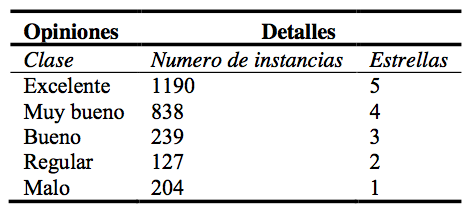
\includegraphics[scale=0.5]{images/tabla_1.png}
\caption{Descripción del corpus de reseñas comerciales}
\end{figure}

\end{frame}

%%%%%%%%%%%%%%%%%%%%%%%%
\begin{frame}\frametitle{\normalsize Corpus de opiniones}

\begin{columns}[T] % contents are top vertically aligned


\begin{column}[T]{5cm} % alternative top-align that's better for graphics

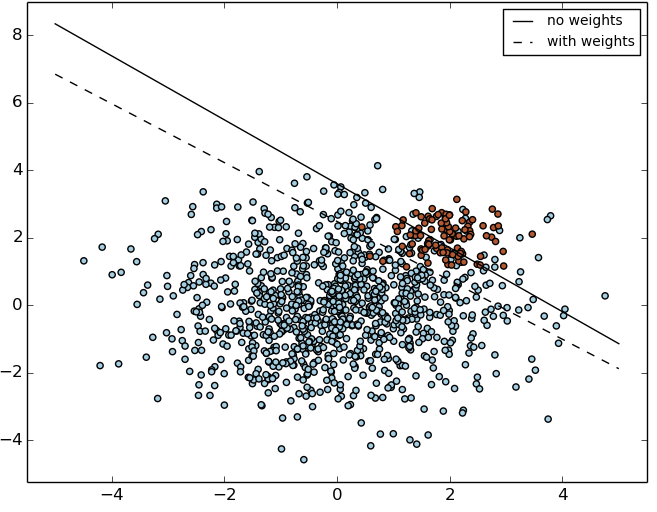
\includegraphics[height=4.3cm]{images/weighted_vs_unweighted.png}
     \end{column}

\begin{column}[T]{6cm} % each column can also be its own environment
En el área de aprendizaje automático se ha considerado el problema del \alert{desequilibrio de clases}.
\setbeamertemplate{itemize items}[square]
\begin{itemize}
\item <1-> Modificación del algoritmo \textit{Sun, Yanmin et al (2007)}.
\item <2-> Asignación de pesos distintos a los ejemplos de entrenamiento, introduciendo diferentes costos a ejemplos positivos y negativos. \textit{Pazzani, Michael et al (1994)}
\item <3-> Muestreo heterogéneo de datos (e.g. bajo-muestreo, sobre-muestreo, metodos hibridos) \textit{Tang, Yuchun et al (2009)}.
\end{itemize}
\end{column}
\end{columns}

\end{frame}


%%%%%%%%%%%%%%%%%%%%

\begin{frame}\frametitle{\normalsize Bigramas afirmativos}

\begin{itemize}
\item <2->\textit{Turney, Peter D. (2002)} \alert{determinó la orientación semántica} mediante una \alert{estrategia} que consiste en:
\begin{enumerate}
\item Extracción de \alert{bigramas} a partir de texto.
\item <3-> Se toman cada bigrama para realizar una búsqueda en la Web empleando el operador NEAR de AltaVista para encontrar cuántos documentos tienen ese bigrama cerca de un \alert{término positivo (excellent)} y de un \alert{término negativo (poor)}.
\item <4->El puntaje para los dos conjuntos se realiza mediante la \alert{medida de información mutua puntual \textit{(PMI)}}.
\begin{itemize}
\item <5->La diferencia de PMI se utiliza para determinar la orientación semántica 
\end{itemize}

\end{enumerate}
\end{itemize}


\end{frame}

%%%%%%%%%%%%%%%%%%%%%%%


\begin{frame}\frametitle{\normalsize Bigramas afirmativos}

\begin{obs}
%\centering
El puntaje $PMI$ de dos palabras $w1$ y $w2$ se obtiene mediante la probabilidad de que las dos palabras aparezcan juntas dividida por la probabilidad de que las dos palabras aparezcan juntas dividida por las probabilidades de cada palabra en forma individual:
\centering
\begin{equation}  PMI(w1,w2) = log\Big[\frac{P(w1,w2)}{P(w2)P(w2)}\Big]
\end{equation}

\end{obs}


\end{frame}
%%%%%%%%%%%%%%%%%%%%%%%%%


\begin{frame}\frametitle{\normalsize Bigramas afirmativos}

La orientación semántica se calculó de la siguiente forma:


\begin{obs}

\begin{equation}
SO(frase) = log \Big[ \frac{hits(Frase \textrm{ NEAR }  excellent) hits (poor)}{hits(frase \textrm{ NEAR } poor) hits(excellent)}\Big]
\end{equation}
\end{obs}


\end{frame}

%%%%%%%%%%%%%%%%%%%%%%%%%%%%%%%%%%%%%%%%%


\begin{frame}\frametitle{\normalsize Bigramas afirmativos}

     \begin{columns}[T] % contents are top vertically aligned
     \begin{column}[T]{5cm} % each column can also be its own environment
    La orientación semántica de bigramas fue utilizada para determinar la orientación semántica de opiniones completas.
    \begin{itemize}
    \item <2-> Turney tomó 410 comentarios de \textit{epinions.com}
    \item <3-> Los resultados oscilaron entre el 66\% y 84\% de precisión.
    \end{itemize}
     \end{column}
     \begin{column}[T]{5cm} % alternative top-align that's better for graphics
\centering
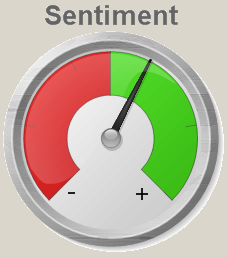
\includegraphics[height=3cm]{images/sentimiento.png}
     \end{column}
     \end{columns}
\end{frame}



\begin{frame}\frametitle{\normalsize Bigramas afirmativos}

\begin{alertblock}{Conclusión}
Los bigramas morfosintácticos  son una buena característica para métodos no supervisados
\begin{itemize}
\item <2->Suponemos que para \textbf{métodos supervisados} podrían ser mejores.
\end{itemize}
\end{alertblock}


\end{frame}

%%%%%%%%%%%%%%%%%%%%%%%%%%%%%%%%%%%%%%%%%%%%%%%
\begin{frame}\frametitle{\normalsize Bigramas afirmativos}
En este trabajo consideramos los siguientes bigramas morfosintácticos como característica para el entrenamiento del \textbf{método supervisado}:
\begin{obs}
Estos bigramas morfosintáticos no corresponden a compuestos obtenidos por un analizador sintáctico.
\end{obs}

\begin{itemize}
\item <2->Sustantivo - adjetivo
\item <3->Verbo - adverbio
\item <4->Adverbio - adjetivo
\item <5->Adjetivo - adverbio
\end{itemize}

\end{frame}


%%%%%%%%%%%%%%%%%%%%%%%%%%%%%%%%%%%%%%%%%


\begin{frame}\frametitle{\normalsize Bigramas afirmativos}

Mediante un conjunto de scripts a partir de la colección de opiniones, se obtienen todas las secuencias de dos palabras cuyas categorías gramaticales completen los patrones antes indicados (\textit{i.e. bigramas}).

\begin{itemize}
\item <2->En el caso sustantivo-adjetivo el programa que extrae estos bigramas comprueba la concordancia en género y número.
\item <3->Para todos los bigramas se extraen no solo las palabras, también los lemas.
\begin{itemize}
\item <4->Esto permite agrupar diversas formas en una sola característica.
\end{itemize}
\end{itemize}

\begin{example}
<5->Por ejemplo:\textit{prenda vaquera} y \textit{prendas vaqueras}, \textit{lavadora nueva} y \textit{lavadoras nuevas}, se agrupan en un solo bigrama para cada par.
\end{example}

\end{frame}

%%%%%%%%%%%%%%%%%%%%%%%%%%%%%%%%%%%%%%%%%%%%

\begin{frame}\frametitle{\normalsize Bigramas afirmativos}

\begin{itemize}
\item <2->Bigramas adverbio-adjetivo y adjetivo-adverbio.
\begin{itemize}
\item <3->Aunque en Español la forma adverbio-adjetivo es común también encontramos adjetivo-adverbio
\begin{example}<4->

Adjetivo-adverbio: \textit{\textbf{poco lento}}\\
Adverbio-adjetivo: \textit{\textbf{más eficiente}}
\end{example}
\end{itemize}
\end{itemize}

\end{frame}



\subsection{Clasificación}

%%%%%%%%%%%%%%%%%%%%%%%%%%%%%%%%%%%%%%%%%%%%%%
\section{Aprendizaje automático}
\begin{frame}\frametitle{\normalsize Clasificación}

\begin{exampleblock}{Modelo}<2->
Máquinas de soporte vectorial:
modelos de aprendizaje supervisado para analizar patrones, usados para clasificación y análisis de regresión.

\begin{itemize}
\item <2->Gran variedad de \textbf{funciones kernel}.
\item <3->Generalizar en parecencia de muchas. características, usando funciones de nuestro espacio de hipótesis.
\item <4->Uso de heurísticas como \textbf{Grid Search} para la optimización de \textbf{hiper parámetros}. 

\end{itemize}
\end{exampleblock}


\end{frame}


%%%%%%%%%%%%%%%%%%%%%%%%%%%%%%%%%%%%%%%%%%
\begin{frame}\frametitle{\normalsize Clasificación}

Para una tarea de clasificación es necesario separar los datos entre \alert{conjunto de entrenamiento} y \alert{conjunto de prueba}:

\begin{itemize}
\item <2->En nuestro caso separamos el corpus de opiniones en 70\% para entrenamiento y 30\% para prueba. 
\item <3->Cada ejemplo o instancia se asocia a una clase, categoría o etiqueta 

\begin{itemize}
\item <4->70\% de los datos de entrenamiento fueron etiquetados con la clase correspondiente
\item <5->Mientras que el 30\% de los datos no se les asignó etiqueta.

\end{itemize}

\end{itemize}

\end{frame}
%%%%%%%%%%%%%%%%%%%%%%%%%%%%%%%%%%%%%%%%%%%

\subsection{Preprocesamiento de datos}

\begin{frame}\frametitle{\normalsize Preprocesamiento de datos}

Una de las ventajas de usar un lenguaje de propósito general como Python es la gran cantidad de bibliotecas robustas para implementar distintos métodos y manipular datos.

\begin{figure}
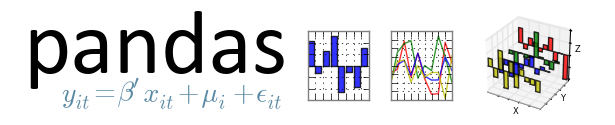
\includegraphics[scale=0.6]{images/pandas_logo.png}
\caption{pandas (Python for data analysis)}
\end{figure}

\end{frame}

%%%%%%%%%%%%%%%%%%%%%%%%%%%%%%%%%%%%%%%%%%%%%%

\subsection{Sistema}

\begin{frame}\frametitle{Sistema}

Para resolver este problema de clasificación, decidimos usar un algoritmo supervisado. La clasificación se hizo mediante SVM para el caso multiclase:
\begin{itemize}
\item <2->Fuertes bases teóricas
\item <3->Algoritmos de aprendizaje que tienen la capacidad de aprender independientemente de la dimensionalidad del espacio de características.
\end{itemize}

\begin{obs}<4->
El objetivo de las SVM es producir un modelo basado en los datos de entrenamiento que prediga las clases o categorías de un conjunto nuevo de instancias, mediante la generación de un hiperplano en un espacio de dimensión infinita.
\end{obs}

\end{frame}


%%%%%%%%%%%%%%%%%%%%%%%%%%%%%%%%%%%%%

\begin{frame}\frametitle{Sistema}

Las SVM funcionan para clasificar texto \footnote{\textit{Joachims, Thorsten. Text categorization with support vector machines: Learning with
many relevant features. Springer (1998).}}:

\begin{itemize}
\item <2->Cuando se clasifica texto se trabaja con espacios de alta dimensión
\item <3->Pocas características irrelevantes, representaciones vectoriales dispersas 
\item <4->Mayor parte de los problemas de clasificación de \alert{texto} son \alert{linealmente separables}.
\end{itemize}


\end{frame}

%%%%%%%%%%%%%%%%%%%%%%%%%%%%%%%%%%%%%%%

\section{Experimentos}
\subsection{Experimentos}
\begin{frame}\frametitle{Experimentos}

\begin{columns}[T] % contents are top vertically aligned
\begin{column}[T]{6cm} % each column can also be its own environment

El entrenamiento de SVM fue realizado empleando la herramienta scikit-learn:
     \setbeamertemplate{itemize items}[square]
  \begin{itemize}
  \item <2->Una biblioteca de código abierto y propósito general.
  \item <3-> Implementa una gran variedad de algoritmos de aprendizaje automático.
  \item <4-> Al igual que otras bibliotecas incorpora o envuelve a la biblioteca de C++ LibSVM.

  
  
  
  \end{itemize}
     \end{column}
     \begin{column}[T]{5cm} % alternative top-align that's better for graphics
          
\includegraphics[height=4cm,scale=0.1]{images/scikit.png}
     \end{column}
     \end{columns}

\end{frame}

%%%%%%%%%%%%%%%%%%%%%%%%%%%%%%%%%%%%%%%%%%%%
\subsection{El truco del kernel}

\begin{frame}\frametitle{El truco del kernel}


\begin{figure}
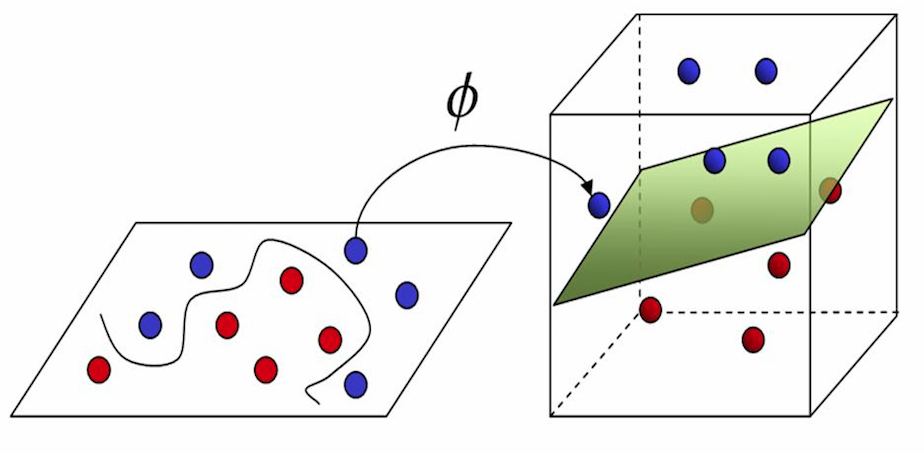
\includegraphics[scale=0.3]{images/truco.png}
\caption{Truco del kernel}
\end{figure}
\end{frame}

%%%%%%%%%%%%%%%%%%%%%%%%%%%%%%%%%%%%%%%%%%%


\begin{frame}\frametitle{El truco del kernel}
Distintas funciones kernel:
\begin{itemize}
\item <2->RBF (\textit{Función de base radial})
\begin{equation} k(x,y)= exp (\gamma ||x-y||^2)
\end{equation}
\item <3->Kernel polinomial \begin{equation}
k(x,y)=(\alpha x^\intercal T y + c)^d
\end{equation}
\item <4-> Kernel lineal
\begin{equation}
k(x,y)=x^\intercal T y + c
\end{equation}
\end{itemize}

\end{frame}

%%%%%%%%%%%%%%%%%%%%%%%%%%%%%%%%%%%%%%%%%%%%%%%
\subsection{Evaluación}
\begin{frame}\frametitle{Evaluación}

\begin{itemize}
\item \textbf{Exactitud:}\\
Calcula el subconjunto de la precisión del conjunto de etiquetas predichas para una muestra que exactamente corresponden al conjunto de etiquetas del conjunto de entrenamiento.\\
 \item \textbf{F1-score:}\\
Promedio balanceado entre la precisión y el recall, %una F1-score alcanza su mejor valor en 1 y su peor valor en 0. La contribución relativa de precisión y recall al F1-score son iguales.\\
 \item \textbf{Score:}\\
Se refiere a la media de la precisión, dados los datos y etiquetas de prueba.\\
  
\end{itemize}


\end{frame}


%%%%%%%%%%%%%%%%%%%%%%%%%%%%%%%%%%%%%%%%%%%%%%%%

\begin{frame}\frametitle{Evaluación}
\begin{itemize}
\item \textbf{Recall:}\\
Es la capacidad que tiene un estimador de encontrar todas las muestras positivas. El recall es el radio $\frac{t_p}{t_p+f_n}$ donde $t_p$ es el numero de verdaderos positivos y $f_n$ es el numero de falsos negativos.\\
  \item \textbf{Precisión:}\\
Intuitivamente podemos decir que es la capacidad que tiene un estimador de no etiquetar como positiva una muestra que es negativa. El radio de precisión: $\frac{t_p}{t_p+f_p}$ donde $t_p$ es el numero de verdaderos positivos y $f_p$ el numero de falsos positivos.\\
  
\end{itemize}
\end{frame}
%%%%%%%%%%%%%%%%%%%%%%%%%%%%%%%%%%%%%%%%%%%%%%

\begin{frame}\frametitle{Evaluación}
\begin{itemize}

\item \textbf{Perdida de Hamming:}\\
  En clasificación multiclase, la perdida de Hamming corresponde a la distancia de Hamming entre el subconjunto de instancias de entrenamiento y el subconjunto de instancias predichas. %Esto es equivalente al subconjunto de la funcion perdida cero-uno, por lo que la perdida de Hamming es la fracción promedio de etiquetas que fueron predecidas de forma incorrecta.\\
  \item \textbf{Similaridad de Jaccard:}\\
Útil para comparar el conjunto de etiquetas predichas para una muestra correspondiente a un conjunto de etiquetas en los datos de entrenamiento.\\
  \item \textbf{F-Beta Score:}\\
  Esta métrica es la media harmónica balanceada entre la precisión y el recall, alcanzando su óptimo valor en 1 y su peor valor en 0.
\end{itemize}
\end{frame}

%%%%%%%%%%%%%%%%%%%%%%%%%%%%%%%%%%%%%%%%%%%%%%

\subsection{Grid search}
\begin{frame}\frametitle{Grid search}


\begin{columns}[T] % contents are top vertically aligned
\begin{column}[T]{6cm} % each column can also be its own environment

Las SVM son sensibles al conjunto de hiperparametros con las que son entrenados.
     \setbeamertemplate{itemize items}[square]
  \begin{itemize}
  \item <2->Un estimador
  \item <3->Un espacio de parámetros
  \item <4->Un método para buscar o muestrear candidatos
  \item <5->Un esquema de validación cruzada
  \end{itemize}
     \end{column}
     \begin{column}[T]{5.5cm} % alternative top-align that's better for graphics
          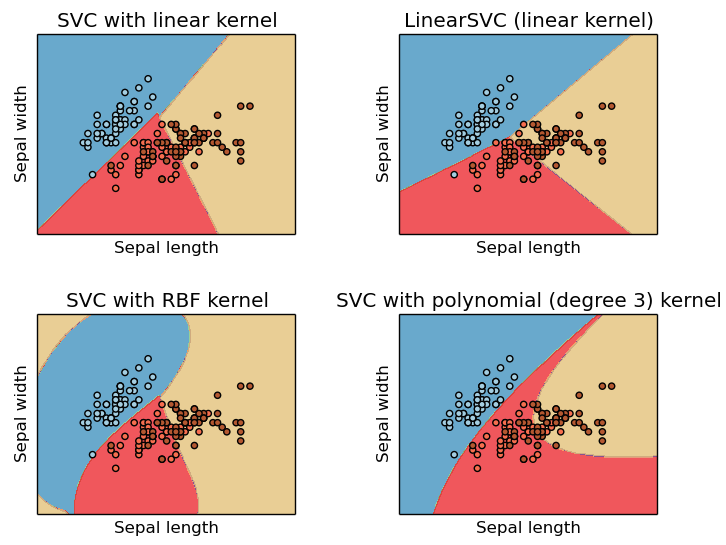
\includegraphics[height=3.0cm,scale=0.1]{images/svm_image.png}
     \end{column}
     \end{columns}
     

\end{frame}
%%%%%%%%%%%%%%%%%%%%%%%%%%%%%%%%%%%%%%%%%%%%
\begin{frame}\frametitle{Grid search}


\begin{obs}
Una \textbf{\textit{Grid search}} es una búsqueda exhaustiva a través de un subconjunto del espacio de hiper-parámetros de un algoritmo de aprendizaje.
\end{obs}

\end{frame}
%%%%%%%%%%%%%%%%%%%%%%%%%%%%%%%%%%%%%%%%

\subsection{Evaluando el rendimiento base}
%%%%%%%%%%%%%%%%%%%%%%%%%%%%%%%%%%%%%%%%%%%%%%

\begin{frame}\frametitle{Evaluando el rendimiento base}

\begin{obs}
Evaluar la tasa base de éxito puede aportar un valor mínimo que otro estimador debe superar.(\textit{e.g. tareas de clasificación}).
\end{obs}

\end{frame}

%%%%%%%%%%%%%%%%%%%%%%%%%%%%%%%%%%%%%%%%%%%%%%%

\begin{frame}\frametitle{Evaluando el rendimiento base}



\begin{columns}[T] % contents are top vertically aligned


\begin{column}[T]{5cm} % alternative top-align that's better for graphics

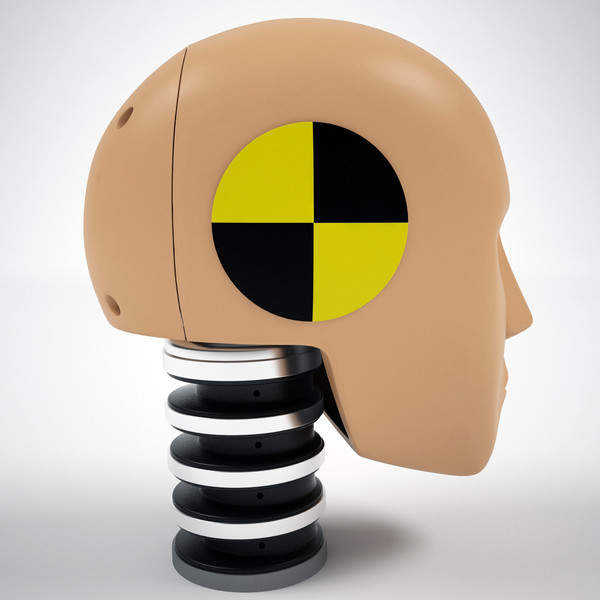
\includegraphics[height=4.3cm]{images/dummy.jpg}
     \end{column}

\begin{column}[T]{6cm} % each column can also be its own environment
Para comparar el resultado usamos un clasificador que usa estrategias simples:
\setbeamertemplate{itemize items}[square]
\begin{itemize}
\item <1-> Es aleatorio.
\item <2-> Siempre predice la etiqueta más frecuente en el conjunto de entrenamiento.
\end{itemize}
\begin{obs}<3->
Esto es equivalente a usar la estrategia de clasificación más frecuente que implementa la herramienta con la que se hizo el entrenamiento.
\end{obs}

\end{column}
\end{columns}


     
\end{frame}
%%%%%%%%%%%%%%%%%%%%%%%%%%%%%%%%%%%%%%%%%%%%%%


\begin{frame}\frametitle{Evaluando el rendimiento base}
Se obtuvieron los siguientes resultados con el sistema base (\textit{i.e. clasificación más frecuente}): 
\begin{itemize}
\item \textit{Exactitud: 0.33}
\item \textit{F1 score: 0.33}
\item \textit{Score:0.32}
\item \textit{Recall: 0.33}
\item \textit{Precisión: 0.32}
\item \textit{Perdida de Hamming: 0.66}
\item \textit{Similaridad de Jaccard: 0.33}
\item \textit{F-Beta score: 0.20}


\end{itemize}

\end{frame}
%%%%%%%%%%%%%%%%%%%%%%%%%%%%%%%%%%%%%%%%
\section{Resultados}
\subsection{Resultados}

\begin{frame}\frametitle{Resultados}
Generamos distintos conjuntos de entrenamiento:
\begin{enumerate}


\item <2->Sustantivo-adjetivo
\begin{itemize}
\item Este bigrama \alert{expresa} atributos sustantivos que corresponden a atributos de \alert{características} del \alert{producto}.
\item Exactitud:82.86 y F-beta: 78.22
\end{itemize}


\item <3->Sustantivo-adjetivo y verbo-adverbio
\begin{itemize}
\item Expresa el modo en que se realiza la \alert{acción descrita por el verbo}.
\item Mejoró un 10\%
\item Exactitud: 92.65 y F-beta: 92.85
\end{itemize}

\item <4->Sustantivo-adjetivo, verbo-adverbio y adverbio-adjetivo
\begin{itemize}
\item Exactitud: 92.30 y F-beta: 93.23
\end{itemize}

\item <5->Sustantivo-adjetivo, verbo-adverbio, adverbio-adjetivo y adjetivo-adverbio

\begin{itemize}
\item No es una estructura lingüística muy usada en Español.
\item \textit{mejor claro}, \textit{super bien}, \textit{perfecto desde\_luego}.

\item Exactitud: 93.12 y F-beta: 94.07

\end{itemize}


\end{enumerate}
\end{frame}

%%%%%%%%%%%%%%%%%%%%%%%%%%%%%%%%%
\begin{frame}\frametitle{Resultados}


\begin{figure}
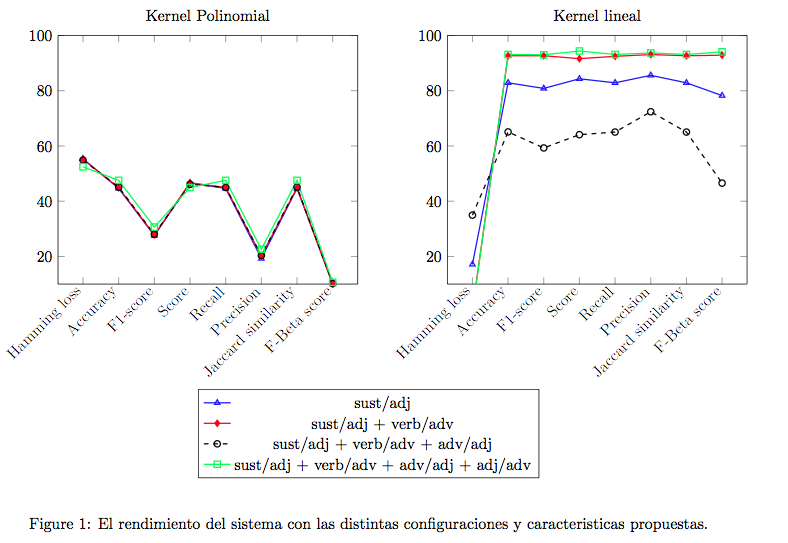
\includegraphics[scale=0.3]{images/plots_2.png}
\caption{Rendimiento del sistema con distintas configuraciones}
\end{figure}

\end{frame}

%%%%%%%%%%%%%%%%%%%%%%%%%%%%%%%%%%%%%%%%%%%
\begin{frame}\frametitle{Resultados}


\begin{itemize}
\item <2->Se han utilizado colecciones de 25 opiniones favorables y 25 opiniones desfavorables para lavadoras con un método no supervisado (\textit{Vilares, David et al 2013}).
\begin{itemize}
\item <3->Precisión de 88 para opiniones negativas y 76 para opiniones positivas.
\end{itemize}
\item <4->Análogamente se han usado SVM para colecciones de opiniones de cine (\textit{Cruz Mata, F. et al 2008}).
\begin{itemize}
\item <5-> Precisión:87.7, Recall:87.63, F1-Score:87.66
\end{itemize}

\end{itemize}
\begin{alertblock}{Conclusión}<6->
Estos resultados muestran que el enfoque propuesto en este trabajo se equipara con el estado del arte de minería de opiniones en español.
\end{alertblock}


\end{frame}


%%%%%%%%%%%%%%%%%%%%%%%%%%%%%%%
\section{Conclusiones}
\subsection{Conclusiones}
\begin{frame}\frametitle{Conclusiones}

\begin{block}{}

\begin{itemize}
\item <2->Examinamos el problema de \textbf{estimar la orientación semántica de opiniones de productos comerciales}, en \textbf{idioma Español}.
\item <3->Exploramos las características de una colección de opiniones 
\item <4->Experimentamos con el uso de \textbf{bigramas de afirmación} como \textbf{características de entrenamiento} para un \textbf{método supervisado} (\emph{Máquinas de soporte vectorial})\\
\end{itemize}
\end{block}



\end{frame}


\subsection[]{}

\begin{frame}\frametitle{COMIA 2015}
		
		%con un \emph{tidy}.\\
		\centering{
		\textbf{\huge¡Gracias por su atención!}\\ 
		\emph{\href{mailto:alonsop@ciencias.unam.mx}{alonsop@ciencias.unam.mx}\\ \href{mailto:sngh@fciencias.unam.mx}{sngh@fciencias.unam.mx}}\\
		}
	%\end{block}
\end{frame}



\end{document}
